% This is the backmatter.tex LaTeX file -- ASP Conference Proceedings backmatter.
% Copyright 2010, Astronomical Society of the Pacific Conference Series
%\documentclass[11pt,twoside]{book}
%\usepackage{../asp2010}

%\begin{document}

\pagestyle{empty}
\null
\setlength{\headheight}{0cm}
\setlength{\headsep}{0cm}
\setlength{\textheight}{21.6cm}
\setlength{\footskip}{0cm}

\begin{center}
{\LARGE \bfseries {ASTRONOMICAL SOCIETY OF THE PACIFIC}\\}
\vspace{1.0cm}
\end{center}

\changelinespacing{1.2}

{\fontfamily{phv}\selectfont 

\begin{wrapfigure}{l}{5.0truecm}
  \vspace{-0.75cm}
  \centering
  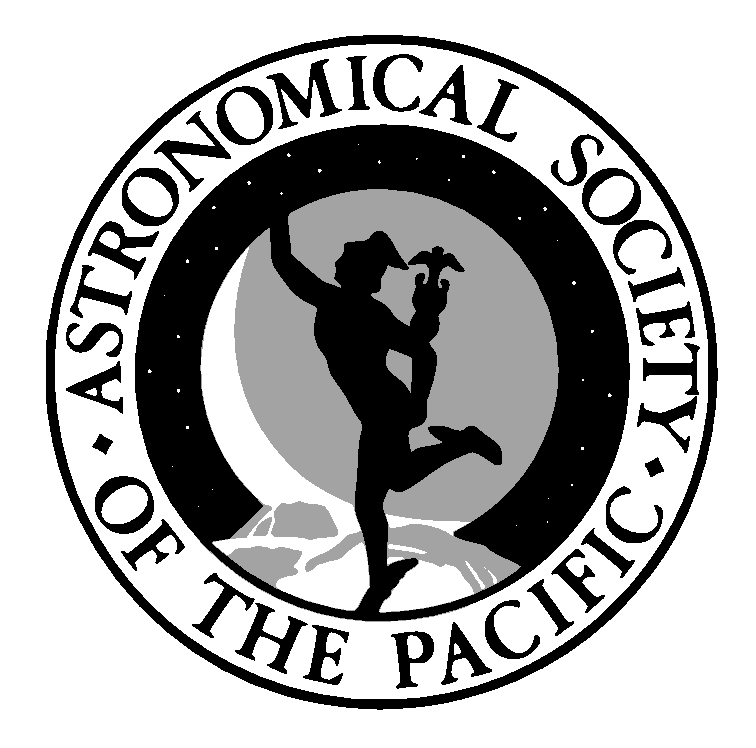
\includegraphics[width=5.0truecm, trim=0 15 0 0]{./frontmatter/logo_bw.eps}
\end{wrapfigure}

\noindent 
\textsc{The Astronomical Society of the Pacific} is an international, 
nonprofit, scientific, and \,\,educational organization. 
Some 120 years ago, on a chilly February evening in San Francisco, 
astronomers from Lick Observatory and members of the Pacific Coast 
Amateur Photographic Association---fresh from viewing the New Year's Day 
total solar eclipse of 1889 a little to the north of the city---met to share 
pictures and experiences. Edward Holden, Lick's first director, complimented 
the amateurs on their service to science and proposed to continue the good 
fellowship through the founding of a Society ``to advance the Science of 
Astronomy, and to diffuse information concerning it.'' The Astronomical 
Society of the Pacific (ASP) was born.

\vspace{5pt}
The ASP's purpose is to increase the understanding and appreciation of 
astronomy by engaging scientists, educators, enthusiasts, and the public to 
advance science and science literacy. The ASP has become the largest 
general astronomy society in the world, with members from over 70 nations.

\vspace{5pt}
The ASP's professional astronomer members are a key component of the
Society. Their desire to share with the public the rich rewards of 
their work permits the ASP to act as a bridge, explaining the mysteries 
of the universe. For these members, the ASP publishes the Publications 
of the Astronomical Society of the Pacific (PASP), a well-respected monthly 
scientific journal. In 1988, Dr. Harold McNamara, the PASP editor at 
the time, founded the ASP Conference Series at Brigham Young University.  
The ASP Conference Series shares recent developments in 
astronomy and astrophysics with the professional astronomy community.

\bigskip

\begin{center}
{\Large To learn how to join the ASP or to make a donation, please visit \url{http://www.astrosociety.org}.}
\end{center}}

\vfill
\eject

% Second page, list of Monographs
\begin{center}
{\Large ASTRONOMICAL SOCIETY OF THE PACIFIC}\\
\vspace{5pt}
{\LARGE \bfseries MONOGRAPH SERIES}\\
\vspace{5pt}
{\small Published by the Astronomical Society of the Pacific}\\
\vspace{5pt}
The ASP Monograph series was established in 1995 to publish select
reference titles. For electronic versions of ASP Monographs, please see
\url{http://www.aspmonographs.org}.
%\end{center}

\noindent\hrulefill
\vspace{1.0em}

%\begin{center}
{\bf INFRARED ATLAS OF THE ARCTURUS SPECTRUM, 0.9-5.3$\mu$m}\\
eds. Kenneth Hinkle, Lloyd Wallace, and William Livingston (1995)\\
ISBN: 1-886733-04-X, e-book ISBN: 978-1-58381-687-5

\vspace{5pt}
{\bf VISIBLE AND NEAR INFRARED ATLAS \\ OF THE ARCTURUS SPECTRUM 3727-9300\AA}\\
eds. Kenneth Hinkle, Lloyd Wallace, Jeff Valenti, and Dianne Harmer (2000)\\
ISBN: 1-58381-037-4, e-book ISBN: 978-1-58381-688-2

\vspace{5pt}
{\bf ULTRAVIOLET ATLAS OF THE ARCTURUS SPECTRUM 1150-3800\AA}\\
eds. Kenneth Hinkle, Lloyd Wallace, Jeff Valenti, and Thomas Ayres (2005)\\
ISBN: 1-58381-204-0, e-book ISBN: 978-1-58381-689-9

\vspace{5pt}
{\bf HANDBOOK OF STAR FORMING REGIONS: VOLUME I\\
THE NORTHERN SKY}\\
ed. Bo Reipurth (2008)\\
ISBN: 978-1-58381-670-7, e-book ISBN: 978-1-58381-677-6

\vspace{5pt}
{\bf HANDBOOK OF STAR FORMING REGIONS: VOLUME II\\ 
THE SOUTHERN SKY}\\
ed. Bo Reipurth (2008)\\
ISBN: 978-1-58381-671-4, e-book ISBN: 978-1-58381-678-3
%\end{center}

%\begin{center}
\hrulefill
\vspace{5pt}

A complete list and electronic versions of ASPCS volumes
may be found at \url{http://www.aspbooks.org}.
\vspace{5pt}

All book orders or inquiries concerning the ASP Conference Series, 
ASP Monographs, or International Astronomical Union Volumes published 
by the ASP should be directed to:\\
\vspace{5pt}
Astronomical Society of the Pacific\\
390 Ashton Avenue\\
San Francisco, CA  94112-1722  USA\\
Phone: 800-335-2624 (within the USA)\\
Phone: 415-337-2126\\
Fax: 415-337-5205\\
Email: \url{service@astrosociety.org}
\vspace{10pt}

For a complete list of ASP publications, please visit
\url{http://www.astrosociety.org}.

\end{center}

%\end{document}
